\documentclass{article}
\usepackage{amsmath,amssymb,amsthm,latexsym,paralist,url}
\usepackage[margin=1in]{geometry}
\usepackage{graphicx}
\graphicspath{ {./} }
\usepackage{tikz}
\usetikzlibrary{arrows,automata}

\theoremstyle{definition}
\newtheorem{problem}{Problem}
\newtheorem*{solution}{Solution}
\newtheorem*{resources}{Resources}


\newcommand{\honor}{\noindent \textbf{Aggie Honor Statement: }On my honor as an Aggie, I have neither
  given nor received any unauthorized aid on any portion of the academic work included in this assignment.
}

 
\newcommand{\checklist}{\noindent\textbf{Checklist:}
Did you...
\begin{compactenum}
\item abide by the Aggie Honor Code?
\item solve all problems?
\item start a new page for each problem?
\item show your work clearly?
\item type your solution?
\item submit a PDF to eCampus?
\end{compactenum}
}

\newcommand{\problemset}[1]{\begin{center}\textbf{Problem Set #1}\end{center}}
\newcommand{\duedate}[1]{\begin{quote}\textbf{Due: #1} on eCampus (\url{ecampus.tamu.edu}). \\You must show your work in order to recieve credit.\end{quote}}
\newcommand{\mysectionnumber}[0]{503}

\title{CSCE 222: Discrete Structures for Computing\\Section \mysectionnumber\\Fall 2016}
\author{Joseph Martinsen}

\begin{document}

\maketitle

\problemset{13: Thanksgiving}

\duedate{27 November 2016 (Sunday) before 11:59 p.m.}

\bigskip

% Hand Turkeys
\begin{problem} (0 points)\\
Make a Hand Turkey (Instructions: \url{http://www.instructables.com/id/Make-a-Hand-Turkey/?ALLSTEPS}).\\
Make your Hand Turkey on a piece of paper.\\
Add a speech bubble to make your turkey say something about your experience in CSCE 222, such as which topic was your favorite, or some (possibly humorous) observation about the course or the instructor.\\
Somewhere on the page, print your name and your age using your non-dominant hand.\\
Scan or take a high-quality picture of your finished Hand Turkey and submit the image as the solution to this problem.\\
\\
Have a Happy Thanksgiving!
\end{problem}

\begin{solution}\ \\
% Figure with caption
\newpage
\begin{figure}[h]
  \begin{center}
    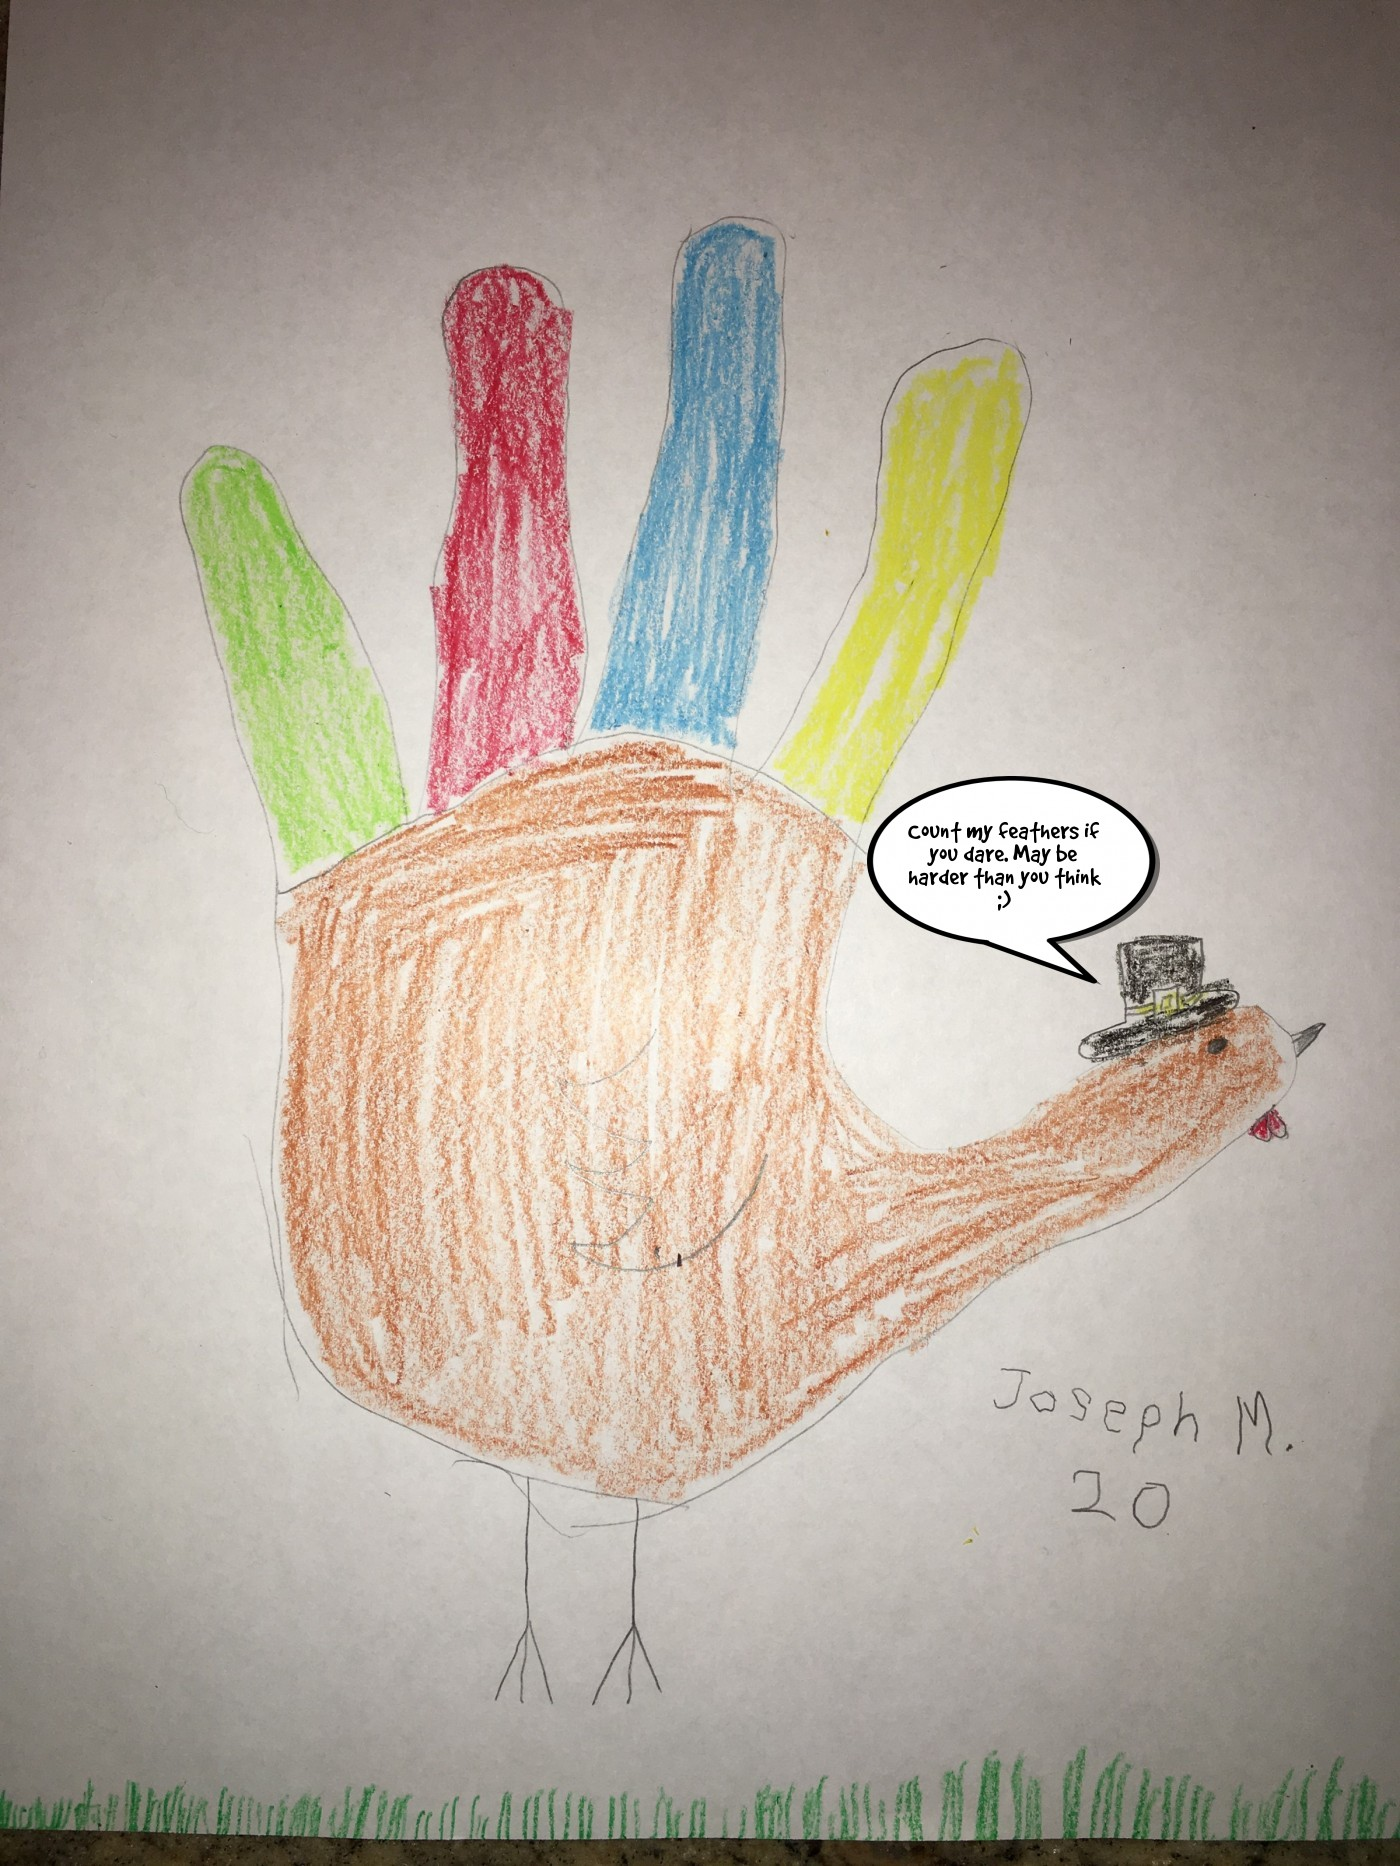
\includegraphics[scale=.25]{pic1.jpg}
  \end{center}
\end{figure}
\end{solution}

\newpage


\bigskip
\honor

\bigskip
\checklist
\end{document}
